\section{ST-structures}
\label{sec:ST-structures}
    
    ST-structures are first introduced by Johansen in \cite{Johansen16STstruct}. They are an extension of \emph{configuration structures} \cite{GlabbeekP95config} and \emph{unrestricted} event structures \cite{GlabbeekP09configStruct}. 
    
    %Configuration structures may be considered the event-based counterpart of transition systems: configurations are the kinds of objects of 0-dimensional ones, vertices, that match the corners of an higher-dimensional automaton, see Figure \ref{fig:st-structure-interleaving-square}. While, event structures may be considered the event-based counterpart of asynchronous transition systems, with a \emph{enabling relation} being similar to the independence relation. However, the enabling relation is defined between sets of events.
    
    \begin{figure}[ht]
        \centering
        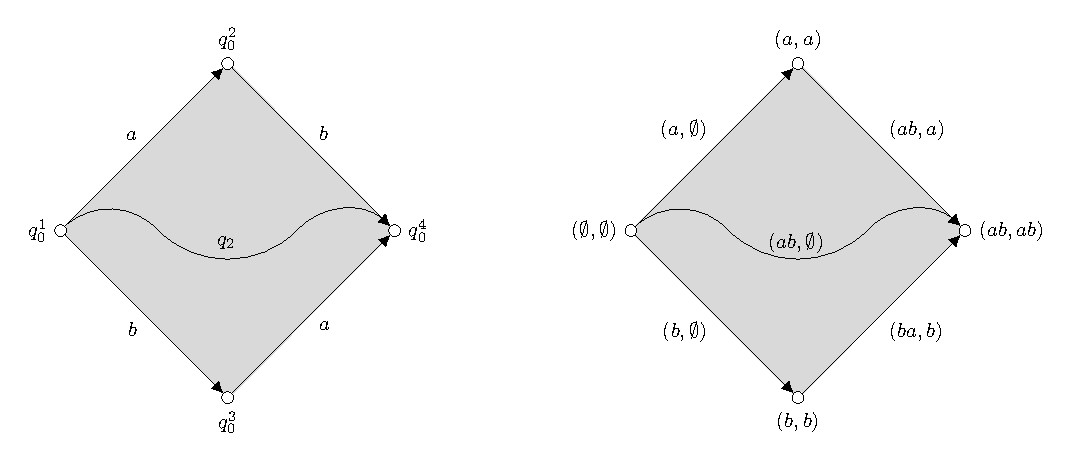
\includegraphics[scale=0.9]{master_thesis/Figures/3.An-introduction-to-non-interleaving-models-for-concurrency/ST-structure/st-structure-interleaving-square.pdf}
         \captionof{figure}[ST-structure]{Example of a higher-dimensional automaton with two concurrent events labelled by $a$ and $b$: with a geometrical picture of the higher-dimensional automaton (left) and of the ST-structure (right).}
        \label{fig:st-structure-interleaving-square}
    \end{figure}
    
    In the case of configuration structures and event structures, we have that the classical notion of concurrency, causality, and conflict are not interdefinable. In the case of higher-dimensional automata these notions can be interdefinable. In Chapter \ref{chap:Relationship with other models of true concurrency}, we relate ST-structures to higher-dimensional automata by identifying a corresponding class of ST-structures with the particular property of \emph{adjacent-closure}. With the adjacent-closure property, ST-structures are able to capture the higher-dimensional case of the notions of concurrency, causality and conflict. We will use the same notation and definitions as Johansen in \cite{Johansen16STstruct}.
    
    \begin{definition}[ST-configuration \cite{Johansen16STstruct}]
        \label{def:st-configuration}
        An ST-configuration over some set $E$ of events is a pair of finite sets ($\mathcal{S},\mathcal{T}$) ($\mathcal{S}, \mathcal{T} \subseteq E$) respecting the property:
        
        \begin{center}
            (start before terminate) $\mathcal{T} \subseteq \mathcal{S}$.
        \end{center}
    \end{definition}
    
    In the following, $\mathcal{S}$ contains the events that have started and $\mathcal{T}$ the events that have terminated. In the current ST-configuration, we see the events $\mathcal{S} \setminus \mathcal{T}$ as being executed \emph{concurrently}. We will call $| \mathcal{S} \setminus \mathcal{T} |$ the concurrent degree of this ST-configuration, similar to how we defined dimensions for higher-dimensional automata. The notion of degree, and dimension, is the main characteristic captured by ST-structures which is found in higher-dimensional automata, but not found in classical event-based models like configuration structures or event structures. In ST-structures, an event can be seen to have started and not terminated yet, capturing the notion of \emph{duration}.
    
%    \ctlong{What is the difference between degree and dimension of higher-dimensional automaton and degree and dimension of ST-structure?}
    
    %The notion of ST-structures by Johansen in \cite{Johansen16STstruct}, that we present in Definition \ref{def:st-structures}, is similar to that of van Glabbeek in \cite[Definition 2.4]{GlabbeekV97splitting} where the ST-structure assumes the existence of a partial order. However, we will present the ST-structure in a similar manner as Johansen by defining the partial order later in the same manner as done for configuration structures \cite{GlabbeekP09configStruct}.
    
    \begin{definition}[ST-structures \cite{Johansen16STstruct}]
        \label{def:st-structures}
        An ST-configuration structure (also called ST-structure) is a tuple $ST$ = ($E, ST, l$) with ST a set of ST-configurations over $E$ satisfying the constraint:
        
        \begin{center}
            if ($\mathcal{S},\mathcal{T}$) $\in$ ST then ($\mathcal{S},\mathcal{S}$) $\in$ $ST$,
        \end{center}
    
    and $l:E$ $\rightarrow \Sigma$ a labelling function with $\Sigma$ the set of labels. we often omit the set of events $E$ from the notation when there is no danger of confusion.
    \end{definition}
    
    Intuitively, the constraint above ensures that every event that is represented, and that has also started, has to be terminated. We denote $\mathbb{S} \mathbb{T}$ as the set of all ST-structures.
    
    \begin{definition}[Stable ST-structures \cite{Johansen16STstruct}]
        \label{def:stable st-structures}
        An ST-structure ($E, ST,l$) is called:
        
        \begin{enumerate}
            \item rooted iff ($\emptyset$,$\emptyset$) $\in ST$;
            \item connected iff for any non-empty ($\mathcal{S},\mathcal{T}$) $\in ST$, either \\
            $\exists$e $\in$ $\mathcal{S}$ : ($\mathcal{S}\setminus e, \mathcal{T}$) $\in ST$ or $\exists$e $\in \mathcal{T}$ : ($\mathcal{S}, \mathcal{T}\setminus e$) $\in ST$;
            \item closed under bounded unions iff for any ($\mathcal{S},\mathcal{T}$),($\mathcal{S}',\mathcal{T}'$),($\mathcal{S}'',\mathcal{T}''$) $\in ST$ if ($\mathcal{S},\mathcal{T}$) $\cup$ ($\mathcal{S}',\mathcal{T}'$) $\subseteq$ ($\mathcal{S}'',\mathcal{T}''$) then ($\mathcal{S},\mathcal{T}$) $\cup$ ($\mathcal{S}',\mathcal{T}'$) $\in ST$;
            \item closed under bounded intersection iff for ($\mathcal{S},\mathcal{T}$),($\mathcal{S}',\mathcal{T}'$),($\mathcal{S}'',\mathcal{T}''$) $\in ST$ if ($\mathcal{S},\mathcal{T}$) $\cup$ ($\mathcal{S}',\mathcal{T}'$) $\subseteq$ ($\mathcal{S}'',\mathcal{T}''$) then ($\mathcal{S},\mathcal{T}$) $\cap$ ($\mathcal{S}',\mathcal{T}'$) $\in ST$;
        \end{enumerate}
        
        An ST-structure is called stable iff it is rooted, connected, and closed under bounded unions and intersections.
    \end{definition}
    
    Stable ST-structures satisfy the properties of being rooted, connected, and closed under bounded unions and intersections. Rooted is where the ST-structure has a ST-configuration that has no events running or terminated. Connected means that for every non-empty configuration, that is, an event has terminated or is running, there must exist another configuration where that event has not started, or terminated, yet. Both closed under bounded union and intersection, are operations that provide configurations that already exist in the ST-structure.
    

    \begin{definition}[Stable ST-structures \cite{Johansen16STstruct}]
    \label{def:st-steps}
        A step between two ST-configurations is defined as either:
        
        \begin{description}
            \item[s-step] $(\mathcal{S},\mathcal{T})\transitions{e}(\mathcal{S}',\mathcal{T}')$ when $\mathcal{T}=\mathcal{T}'$, $\mathcal{S} \subset \mathcal{S}'$, $\mathcal{S}' \setminus \mathcal{S}=\{e\}$; or
            \item[t-step] $(\mathcal{S},\mathcal{T})\transitiont{e}(\mathcal{S}',\mathcal{T}')$ when $\mathcal{S}=\mathcal{S}'$, $\mathcal{T} \subset \mathcal{T}'$, $\mathcal{T}' \setminus \mathcal{T}=\{e\}$.
        \end{description}
        When the type is unimportant we denote a step by \, $\transition{e}$ \, for \, $\transitions{e}\cup\transitiont{e}$. A \emph{path} of an ST-structure, denoted $\pi$, is a sequence of steps, where the end of one is the beginning of the next, in other words,
        
        \[
            \pi\defequal(\mathcal{S},\mathcal{T})\transition{e}(\mathcal{S}',\mathcal{T}')\transition{e'}(\mathcal{S}'',\mathcal{T}'')\dots
        \]

        A path is \emph{rooted} if it starts in $(\emptyset,\emptyset)$.
    \end{definition}

%    \begin{definition}[ST-steps \cite{Johansen16STstruct}]
%        \label{def:st-steps}
%        A step between two ST-configurations is defined as either:
%        
%        \begin{itemize}
%            \item \textbf{s-step:} ($\mathcal{S},\mathcal{T}$)$\xrightarrow[s]{a}$ when $\mathcal{T} = \mathcal{T}', \mathcal{S}' = \mathcal{S} \cup \{e\}, e \notin \mathcal{S}$, and $l(e) = a$; or
%            \item  \textbf{t-step:} ($\mathcal{S},\mathcal{T}$)$\xrightarrow[t]{a}$ when $\mathcal{S} = \mathcal{S}', \mathcal{T}' = \mathcal{T} \cup \{e\}, e \notin \mathcal{T}$, and $l(e) = a$.
%        \end{itemize}

%        when the type is unimportant we denote a step by $\xrightarrow{a}$ for $\xrightarrow[s]{a} \cup \xrightarrow[t]{a}$.
%    \end{definition}
    
    A \emph{computational interpretation} for ST-structures is defined by defining simple steps between ST-configurations, similar to interpretations for other concurrency models like configurations structures. However in \cite[Theorem 3.10]{Johansen16STstruct}, the computational interpretation for ST-structures is shown to be more fine-grained than other models such as configuration structures and event structures, since ST-structures can capture the notion of \emph{duration}.
    
    The notion of duration is similar to what is captured in higher-dimensional automata, but from a state-based perspective. Hence, ST-structures are capable of showing a natural sequence of \emph{observable information} as ST-traces in a similar manner as higher-dimensional automata \cite[Section 7.3]{Glabbeek06HDA}. Following the notion of Johansen in \cite{Johansen16STstruct}, we may consider ST-structures the richest formalisation of observable content for concurrent systems.
    
    \begin{definition}[Paths and traces \cite{Johansen16STstruct}]
        \label{def:paths and traces}
        A path of an ST-structure, denoted $\pi$, is a sequence of steps, where the end of one is the beginning of the next, that is,
        
        \begin{center}
            $\pi \triangleq$ $(\mathcal{S}_{0},\mathcal{T}_{0})\xrightarrow{a}(\mathcal{S}_{1},\mathcal{T}_{1})\xrightarrow{b}(\mathcal{S}_{2},\mathcal{T}_{2})$...    
        \end{center}
        
        A path is rooted if it starts in ($\emptyset$,$\emptyset$). The ST-trace of a rooted path $\pi$, denoted $st(\pi)$, is the sequence of labels of the steps of $\pi$ where each label is annotated as a $a^{0}$ if it labels an s-step or as $a^{n}$ if it labels a t-step. where $n \in  \mathbb{N}$ is determined by counting from the beginning the number of steps until the s-step that has added the event \emph{e} to the $\mathcal{S}$ set, which \emph{e} being the event that has been added to $\mathcal{T}$ in the current t-step.
    \end{definition}
    
    If we consider rooted and connected ST-structures, then the notion of ST-trace matches with the one in \cite[Definition 2.5]{GlabbeekV97splitting} and in \cite[Section 7.3]{Glabbeek06HDA}. Below we define the notion of concurrency and causality for a particular ST-configuration as Johansen in \cite{Johansen16STstruct}.
    
    \begin{definition}[Concurrency and causality \cite{Johansen16STstruct}]
        \label{def:ST concurrency and causality}
        For a particular ST-configuration ($\mathcal{S},\mathcal{T}$) $\in \cat{ST}$ where $e, e' \in \mathcal{S}$ satisfies
        
        \begin{itemize}
            \item \textbf{Concurrency:} $e \parallel e'$ iff there exists $(\mathcal{S}',\mathcal{T}') \subseteq (\mathcal{S},\mathcal{T})$ such that
            \begin{itemize}
                \item $(\mathcal{S}',\mathcal{T}') \in \cat{ST}$, and
                \item $\{e,e'\} \subseteq \mathcal{S}' \setminus \mathcal{T}'$.
            \end{itemize}
            \item \textbf{Causality:} $e < e'$ iff $e \neq e'$ and for any $(\mathcal{S}',\mathcal{T}') \subseteq (\mathcal{S},\mathcal{T})$ such that
            \begin{itemize}
                \item $(\mathcal{S}',\mathcal{T}') \in \cat{ST}$, and
                \item $e' \in \mathcal{S}' \Rightarrow e \in \mathcal{T}'$.
            \end{itemize}
        \end{itemize}
        
        %For a particular ST-configuration ($\mathcal{S},\mathcal{T}$) $\in \cat{ST}$ define the relations of concurrency and causality on the events in $\mathcal{S}$ as:
        
        %\noindent \textbf{concurrency} for $e, e' \in \mathcal{S}$ then $e \parallel e'$ iff exists ($\mathcal{S}',\mathcal{T}'$)$\subseteq$($\mathcal{S},\mathcal{T}$) such that ($\mathcal{S}',\mathcal{T}'$)$\in \cat{ST}$ and ${e,e'} \subseteq \mathcal{S}' \backslash \mathcal{T}'$; 
        
        %\noindent \textbf{causality} for $e, e' \in \mathcal{S}$ then $e < e'$ iff $e \neq e'$ and for any ($\mathcal{S}', \mathcal{T}'$)$\subseteq$($\mathcal{S}, \mathcal{T}$) such that ($\mathcal{S}', \mathcal{T}'$) $\in \cat{ST}$, is the case $e' \in \mathcal{S}' \Rightarrow e \in \mathcal{T}'$.
        
    \end{definition}
    
    \emph{Concurrency} for ST-structures is satisfied if we can find an ST-configuration where two events have started, not yet terminated, and is persistent throughout an execution. Other event-based models such as event structures represent concurrency as having events that are not in conflict and not partial ordered. ST-configurations represent concurrency by providing information about the currently concurrent events. 
    
    %As observed by Johansen in \cite{Johansen16STstruct}, concurrency for ST-structures is sound since each ST-configuration provides information about the currently concurrent events. However, concurrency for ST-configurations do not provide complete information about the concurrency relation in the whole system. Hence, concurrency is not complete for ST-configurations.
    
    \emph{Causality} for an ST-configurations is similar to the way causality is defined as a partial order for configuration structures, such that  causality is a local definition for an ST-configuration.
    
    For an arbitrary ST-structure, concurrency and causality are not interdefinable such that concurrency is the complement of causality, as in the standard way \cite[Definition 5.6]{GlabbeekG01refinement}. If we consider well behaved ST-structures such as stable ST-structures, then concurrency and causality can be seen as interdefinable in the standard way.
    
    \begin{definition}[Conflict \cite{Johansen16STstruct}]
        \label{def:ST-structure conflict}
        For an ST-structure ST the notion of global conflict is defined as a predicate over sets of events $E' \subseteq E$:
        
        \begin{center}
            $\# E'$ iff $\nexists (\mathcal{S},\mathcal{T}) \in ST$ with $E' \subseteq \mathcal{S}$.
        \end{center}
    \end{definition}
    
    In the following, the ST-structure describes conflicting events as a predicate where conflicting events in a ST-structure can never appear in the same configuration. Conflicting events is defined as a general notion on the whole ST-structure, and is considered to be similar to the standard notion of binary conflict for event structures \cite{winskel95modelsCategory}.

    \begin{definition}[Adjacent-closure \cite{Johansen16STstruct}]
        \label{def:ST adjacent-closure}
        We call an ST-structure ST adjacent-closed if the following are respected:
       
       \begin{enumerate}
           \item if $(\mathcal{S},\mathcal{T}), (\mathcal{S} \cup e, \mathcal{T}), (\mathcal{S} \cup \{e,e'\}, \mathcal{T}) \in ST$, with $(e \neq e') \notin \mathcal{S}$,\\
           then $(\mathcal{S} \cup e', \mathcal{T}) \in ST;$
           \item if $(\mathcal{S},\mathcal{T}), (\mathcal{S} \cup e, \mathcal{T}), (\mathcal{S} \cup e, \mathcal{T} \cup e') \in ST$, with $e \notin S \wedge e' \notin \mathcal{T} \wedge e \neq e'$, \\
           then $(\mathcal{S}, \mathcal{T} \cup e') \in ST;$
           \item if $(\mathcal{S},\mathcal{T}), (\mathcal{S} \cup e, \mathcal{T}), (\mathcal{S}, \mathcal{T} \cup e') \in ST$, with $e' \notin \mathcal{S} \wedge e' \notin \mathcal{T} \wedge e \neq e'$, \\
           then $(\mathcal{S} \cup e, \mathcal{T} \cup e') \in ST;$
           \item if $(\mathcal{S},\mathcal{T}), (\mathcal{S}, T \cup e), (\mathcal{S}, T \cup \{e,e'\}) \in ST$, with $(e \neq e') \notin \mathcal{T}$, \\
           then $(\mathcal{S}, \mathcal{T} \cup e') \in ST;$
       \end{enumerate}
    \end{definition}
    
    In the following, adjacent-closure for ST-structure is related to the definition of higher-dimensional automata, in other words, the precubical identities of higher-dimensional automata. In the definition of \emph{adjacent} \cite[Definition 19]{Glabbeek99invitedCONCUR}, the correlation becomes more visible when looking at the homotopy over higher-dimensional automata. The homotopy over higher-dimensional automata essentially define histories of higher-dimensional automata, see Definition \ref{def:histories-for-HDA}. Similarly, the above adjacent-closure on ST-structures makes sure that the histories of ST-configurations are represented.
    
    \begin{definition}[Morphisms of ST-structures \cite{Johansen16STstruct}]
        \label{def:morphisms of ST-structures}
        A morphism $f: ST \rightarrow ST'$ between two ST-structures ST = ($E, ST, l$) and ST' = ($E', ST', l'$) is defined as a partial function on the events, $f: E \rightarrow E'$ which:
        
        \begin{itemize}
            \item preserves ST-configurations, if ($\mathcal{S},\mathcal{T}$) $\in ST$ then $f(\mathcal{S},\mathcal{T}) = (f(\mathcal{S}),f(\mathcal{T})) \in ST'$,
            \item preserves the labelling when defined, that is, $l'(f(e)) = l(e)$ if $f$ is defined for $e$, and
            \item is locally injective and total, that is, for any ($\mathcal{S}, \mathcal{T}$) $\in ST$ the restriction $f\rest S$ i s injective and total.
        \end{itemize}
    \end{definition}
    
    Morphisms of ST-structures are structure-preserving maps such that if $\mathcal{T} \subseteq \mathcal{S}$ then $f(\mathcal{T}) \subseteq f(\mathcal{S})$. If morphisms are not local and total, then morphisms are not guaranteed to preserve steps as shown by Johansen in \cite[Proposition 2.21]{Johansen16STstruct}.
    
    \begin{definition}[Isomorphic ST-structures \cite{Johansen16STstruct}]
        \label{def:isomorphic-ST-structures}
        A function $f$ is an isomorphism of two ST-configurations ($\mathcal{S},\mathcal{T}$)$f$($\mathcal{S}',\mathcal{T}'$) iff $f$ is a bijection between $\mathcal{S}$ and $\mathcal{S}'$ that agrees on the sets $\mathcal{T}$ and $\mathcal{T}'$ (that is, $f \rest T = \mathcal{T}'$). Two ST-structures ST and ST are isomorphic, denoted $ST \cong ST'$, iff there exists a bijection $f$ on their events that is also a morphism between the two ST-structures. 
    \end{definition}
    
%    By considering morphisms of ST-structures to be bijections, we are able to consider two ST-structures isomorphic.
    
    \begin{definition}[Category of ST \cite{Johansen16STstruct}]
        \label{def:category of ST}
        We can define a category $\allST$ to have objects ST-structures and the morphisms from Definition \ref{def:morphisms of ST-structures} because composition of morphisms is well defined for any ST-structure there exists a unique identity morphism which is the total function taking an event to itself.
    \end{definition}
    
%    \begin{definition}[hh-bisimulation for ST-structures \cite{Johansen16STstruct}]
%        \label{def:hh-bisimulation for ST-structures}
%        For two ST-structures ST and ST', a relation $R \subseteq ST \times ST' \times P(ST \times ST')$ is called history preserving bisimulation between ST and ST' iff $(\emptyset, \emptyset, \emptyset) \in R$ and whenever $((\mathcal{S},\mathcal{T}),(\mathcal{S}',\mathcal{T}'),f) \in R$ then
        
%        \begin{enumerate}
%            \item f is an isomoprhism between ($\mathcal{S},\mathcal{T}$) and ($\mathcal{S}',\mathcal{T}'$); and
%            \item if ($\mathcal{S},\mathcal{T}$) $\xrightarrow[]{a}$ ($\mathcal{S}_{a},\mathcal{T}_{a}$) in $ST$, then there exists ($\mathcal{S}'_{a},\mathcal{T}'_{a}$) $\in ST'$ and $f'$ extending f (i.e., $f' \rest{(S,T)}$ = f with ($\mathcal{S}',\mathcal{T}'$) $\xrightarrow[]{a}$ ($\mathcal{S}'_{a},\mathcal{T}'_{a}$) and (($\mathcal{S}_{a},\mathcal{T}_{a}$),($\mathcal{S}'_{a},\mathcal{T}'_{a}$),$f'$) $\in R;$ and
%            \item if ($\mathcal{S}',\mathcal{T}'$) $\xrightarrow[]{a}$ ($\mathcal{S}'_{a},\mathcal{T}'_{a}$) $in ST'$, then there exists ($\mathcal{S}_{a},\mathcal{T}_{a}$) $\in ST$ and $f'$ extending f with ($\mathcal{S},\mathcal{T}$) $\xrightarrow[]{a}$ ($\mathcal{S}_{a},\mathcal{T}_{a}$) and (($\mathcal{S}_{a},\mathcal{T}_{a}$),($\mathcal{S}'_{a},\mathcal{T}'_{a}$),$f'$) $\in R$.
%        \end{enumerate}
        
%        R is moreover called hereditary if the following back condition holds:
        
%        \begin{enumerate}
%            \setcounter{enumi}{3}
%            \item if ($\mathcal{S}_{a},\mathcal{T}_{a}$) $\xrightarrow[]{a}$ ($\mathcal{S},\mathcal{T}$) in $ST$, then there exists ($\mathcal{S}'_{a},\mathcal{T}'_{a}$) $\in ST'$ and $f'$ with $f \rest{(S_{a},T_{a})}$ = f' and ($\mathcal{S}'_{a},\mathcal{T}'_{a}$) $\xrightarrow[]{a}$ ($\mathcal{S}',\mathcal{T}'$) and (($\mathcal{S}_{a},\mathcal{T}_{a}$),($\mathcal{S}'_{a},\mathcal{T}'_{a}$),$f'$) $\in R$.
%            \item if ($\mathcal{S}'_{a},\mathcal{T}'_{a}$) $\xrightarrow[]{a}$ ($\mathcal{S}',\mathcal{T}'$) in ST', then there exists ($\mathcal{S}_{a},\mathcal{T}_{a}$) $\in ST$ and $f'$ with $f \rest{(S'_{a},T'_{a})}$ = f' and ($\mathcal{S}_{a},\mathcal{T}_{a}$) $\xrightarrow[]{a}$ ($\mathcal{S},\mathcal{T}$) and (($\mathcal{S}_{a},\mathcal{T}_{a}$),($\mathcal{S}'_{a},\mathcal{T}'_{a}$),$f'$) $\in R$.
%        \end{enumerate}
        
%        A history preserving bisimulation between two ST-structures is denoted $ST h ST'$, and a hereditary one is denoted $ST hh ST'$. We usually abbreviate to hh-bisimulation.
%    \end{definition}
    
%    \ctlong{Explain the bisimulation for ST-structures.}
  
%    Because of symmetry of the requirements for history preserving bisimulation (i.e., the points 2 and 3 above), the two conditions for hereditary are redundant together, and we could well use only one of them. In our proofs we will consider only condition 4. \ct{reword!}
    
    %As introduced by Johansen in \cite{Johansen16STstruct}, ST-structures are the event-based counterpart of higher-dimensional automata. However, as we present in Chapter \ref{chap:Relationship with other models of true concurrency}, isomorphic higher-dimensional automata are interpreted as non-isomorphic ST-structures. Hence, there is not an embedding, that is, an injective morphism, from $\allST$ to $\allHDA$. We also show in Figure \ref{fig:Unfolding-HDA} that non-isomorphic higher-dimensional automata interpreted as ST-structures become isomorphic ST-structures, meaning there is not an embedding from $\allHDA$ to $\allST$. Hence, higher-dimensional automata are neither more, or less, expressive than ST-structures. Chu spaces and sculptures are introduced as models to reconcile the relationship between ST-structures and higher-dimensional automata, which we will introduce in Section \ref{sec:Chu-spaces-and-ST-structures} and Section \ref{sec:sculpture-and-st-structure}
    
    %Leading to the investigation of the sculpting method for higher dimensional automata, which we present in Chapter \ref{chap:sculpting-in-concurrency}.
    
    %Before introducing sculptures, we will review Chu spaces which is a model that can capture the event-state duality of higher-dimensional automata and ST-structures.
    
    %Furthermore, we will attempt to show that ST-structures are isomorphic to Chu spaces over $3$.
    
    
%    \ctlong{There needs to be a nice transition from ST-structures to Chu spaces. This should come in the form that we will consider Chu spaces over 3 isomorphic to ST-structures. Showing a nice translation between these models and building up to the method of sculpting for higher-dimensional automata.}
   % \ctlong{CONTINUE FROM HERE!!}
    
    %ST-structures\ct{citation} have been introduced as a natural extension of configuration structures\ct{citation} to form the event-based counterpart of higher-dimensional automata. We review here only relevant definitions 


    %\ctlong{Provide the different necessary formulation of describing ST-structures such that we can show the problem of transforming a ST-structure to an higher-dimensional automaton later in the paper. Need to equipped all the necessary tools before this.}
    
    
    
    %%%%% OLD STUFF BELOW!
    
    
    %   Intuitively S contains the events that have started and T the events that have terminated. Therefore, we see the events in S$\setminus$T as being executed \emph{concurrently} in the current ST-configuration. We call their numbers |S$\setminus$T| the concurrency degree of this ST-configuration. An event can be started (i.e., running) but not terminated yet. This notion of seeing events while running but not terminated, is a key aspect captured by ST-structures, and it is also found in higher-dimensional automata, but not in classical event-based models like configuration structures or event structures
    
    
    %%%% ST-structures paper by Christian
    %We define ST-structures below showing that they are a natural extension of configuration structures \cite{GlabbeekP09configStruct}, and define related notions that stem from the latter. The classical notions of concurrency, causality, and conflict are not interdefinable as in the case of event structures or stable configuration structures; but are more loose, as in the case with higher-dimensional automata. In Chapter \ref{chap:Relationship with other models of true concurrency} we relate ST-structures also to higher-dimensional automata by identifying a corresponding class of ST-structures, that is, with the particular property of adjacent-closure. We also define the class of stable ST-structures and relate this with their counterpart in stable configuration structures. We define the (hereditary) history preserving bisimulation in the context of ST-structures, which when stability is imposed on adjacent-closed ST-structures it corresponds to the same bisimulation for stable configuration structures. We will define action refinement for ST-structures and investigate properties of it, like being preserved under the above bisimulation, or that it preserves the properties of the refined ST-structures.
    
    %\begin{definition}[ST-configuration]
    %    \label{def:st-configuration}
    %    An ST-configuration over some set E of events i a pair of finite sets (S,T) (i.e., S, T $\subseteq$ E) respecting the property:
    %    
    %    \begin{center}
    %        (start before terminate) T $\subseteq$ S.
    %    \end{center}
    %\end{definition}
    
   % Intuitively S contains the events that have started and T the events that have terminated. Therefore, we see the events in S$\setminus$T as being executed \emph{concurrently} in the current ST-configuration. We call their numbers |S$\setminus$T| the concurrency degree of this ST-configuration. An event can be started (i.e., running) but not terminated yet. This notion of seeing events while running but not terminated, is a key aspect captured by ST-structures, and it is also found in higher-dimensional automata, but not in classical event-based models like configuration structures or event structures.
   
    %Define the dimension of an ST-configuration to be |(S,T)| = |S| + |T|. Unions and intersections of ST-configurations are considered pairwise.
    
   % The notion of ST-structures is very close to that of [16, Def.2.4] only that here we do not presuppose the existence of a partial order, but we define it later, in the same style as done for configuration structures[9].
    
   % \begin{definition}[ST-structures \cite{Johansen16STstruct}]
   %     \label{def:st-structures}
   %     An ST-configuration structures (also called ST-structure) is a tuple ST = (E, ST, l) with ST a set of ST-configurations over E satisfying the constraint:
        
   %     \begin{center}
   %         if (S,T) $\in$ ST then (S,S) $\in$ ST,  \ct{mark as constraint (1)}  
   %     \end{center}
    
   % and l:E $\rightarrow \Sigma$ a labelling function with $\Sigma$ the set of labels. we often omit the set of events E from the notation when there is no danger of confusion.
  %  \end{definition}
    
   % The constraint (1) above is a closure, ensuring that we do not represent events that are started but never terminated. The set of all ST-structures is denoted  $\mathbb{S} \mathbb{T}$.
    
   % \begin{definition}[stable ST-structures \cite{Johansen16STstruct}]
   %     \label{def:stable st-structures}
   %     An ST-structure (ST,l) is called:
        
   %     \begin{enumerate}
   %         \item rooted iff ($\emptyset$,$\emptyset$) $\in$ ST;
   %         \item connected iff for any non-empty (S,T) $\in$ ST, either \\
   %         $\exists$e $\in$ S : (S$\setminus$e, T) $\in$ ST or $\exists$e $\in$ T : (S, T$\setminus$e) $\in$ ST;
   %         \item closed under bounded unions iff for any (S,T),(S',T'),(S'',T'') $\in$ ST if (S,T) $\cup$ (S',T') $\subseteq$ (S'',T'') then (S,T) $\cup$ (S',T') $in$ ST;
   %         \item closed under bounded intersection iff for (S,T),(S',T'),(S'',T'') $\in$ ST if (S,T) $\cup$ (S',T') $\subseteq$ (S'',T'') then (S,T) $\cap$ (S',T') $in$ ST;
   %     \end{enumerate}
        
   %     An ST-structure is called stable iff it is rooted, connected, and closed under bounded unions and intersections.
  %  \end{definition}
    
  %  We define a computational interpretation for ST-structures by defining simple steps between ST-configurations. Other computational interpretations could be imagined, like the more complex steps defined for STC-structures in [def 6.5]. Our choice is similar to interpretations existing for other concurrency models, like configuration structures. We give results below like Theorem [Th 3.10], meant to show that this computational interpretation is more fine-grained than for other models that ST-structures are compared with. Intuitively, opposed to standard event-based models, the computational interpretation of ST-structures naturally captures the "during" aspect of the events, that is, what happens while an event is executing (before it has finished). The model of higher-dimensional automata do the same job but in the state-based setting. Moreover, action refinement and bisimulation are well behaved wrt. this interpretation. Besides, ST-structures exhibit a natural \emph{observable information} (on the same lines as for higher-dimensional automata) as ST-traces which, cf.[3, Sec 7.3], constitute the best formalization of observable content for concurrent systems.
    
  %  \begin{definition}[ST-steps \cite{Johansen16STstruct}]
  %      \label{def:st-steps}
  %      A step between two ST-configurations is defined as either: \\
        
  %      \textbf{s-step:} (S,T)$\xrightarrow[s]{a}$ when T = T', S' = S$\cup$\{e\}, $e \notin$ S, and l(e) = a; or \\
        
   %     \textbf{t-step:} (S,T)$\xrightarrow[t]{a}$ when S = S', T' = T$\cup$\{e\}, $e \notin$ T, and l(e) = a. \\
        
    %    when the type is unimportant we denote a step by $\xrightarrow{a}$ for $\xrightarrow[s]{a} \cup \xrightarrow[t]{a}$.
   % \end{definition}
    
   % \begin{definition}[paths and traces \cite{Johansen16STstruct}]
   %     \label{def:paths and traces}
   %     A path of an ST-structure, denoted $\pi$, is a sequence of steps, where the end of one is the beginning of the next, that is,
        
   %     \begin{center}
    %        $\pi \triangleq$ $(S_{0},T_{0})\xrightarrow{a}(S_{1},T_{1})\xrightarrow{b}(S_{2},T_{2})$...    
   %     \end{center}
        
  %      A path is rooted if it starts in ($\emptyset$,$\emptyset$). The ST-trace of a rooted path $\pi$, denoted $st(\pi)$, is the sequence of labels of the steps of $\pi$ where each label is annotated as a $a^{0}$ if it labels an s-step or as $a^{n}$ if it labels a t-step. where $n \in  \mathbb{N}$ is determined by counting from the beginning the number of steps until the s-step that has added the event \emph{e} to the S set, which \emph{e} being the event that has been added to T in the current t-step.
        
    %\end{definition}
    
    % For rooted and connected ST-structures the notion of ST-trace conforms with the one defined in \cite[def.2.5]{GlabbeekV97splitting} or \cite[sec.7.3]{Glabbeek06higher-dimensional automaton}.
    
    %\begin{definition}[concurrency and causality \cite{Johansen16STstruct}]
    %   \label{def:ST concurrency and causality}
    %    For a particular ST-configuration (S,T) $\in \cat{ST}$ define the relations of concurrency and causality on the events in S as:
        
   %     \noindent \textbf{concurrency} for e, e' $\in$ S then e$\parallel$e' iff exists (S',T')$\subseteq$(S,T) s.t. (S',T')$\in \cat{ST}$ and ${e,e'} \subseteq S' \backslash T'$; 
        
%        \noindent \textbf{causality} for e, e' $\in$ S then e < e' iff e $\neq e' and for any (S',T')$\subseteq$(S,T) s.t. (S',T')$\in \cat{ST}$, is the case e' $\in$ S' $\Rightarrow$ e $\in$ T'.
   % \end{definition}
  %  \ctlong{Fix the definition above. Commented out Section.}
    
    %ST-structures represent \emph{concurrency} in a way that is different than other event-based models in the sense that each ST-configuration gives information about the currently concurrent events, and this information is persistent throughout the whole execution. Two events are considered concurrent wrt. a particular ST-configuration if and only if at some point in the past (i.e., in some sub-configuration) both events appeared as executing (i.e., in S') and none was terminated yet(i.e., not in T'); they were both executing concurrently. In event structures or configuration structures in order to decide whether two events are concurrent one needs to look at many configurations or many events to decide this. For example, in event structures the concurrency is defined as not being dependent nor conflicting; which requires to inspect all configurations to decide. An ST-configuration does not give complete information about the concurrency relation in the whole system. In consequence one could view the information about concurrency that an ST-configuration provides as being sound but not complete.
    
    %The above two notions of concurrency and causality are defined for one particular ST-configuration; in consequence one could emphasize this by indexing the relation symbol by the particular ST-configuration (similar to what is done in \cite[sec.5.3]{GlabbeekG01refinement}, but the aesthetics would not be so nice in our case.
    
    %This local definition of \emph{causality} for an ST-configuration is in the tradition of viewing causality as a partial order (in fact this definition makes a partial order on the ST-configuration when the ST-structure is rooted and connected).
    
    %In ST-structures we can look at when an event is started and when it terminates. In consequence, an intuitive understanding of causality is that an event \emph{e is a cause of e'} if and only if in all previous ST-configurations, e' is never started without e having terminated. In other words, whenever during the run of the system up to the current ST-configuration, the event e' is supposed to be started (i.e., $e' \in S'$), any event e on which it depends should have been terminated already (i.e., $e \in T'$).
    
    %The definition of event structures from \cite{GlabbeekP09configStruct} uses a \emph{dependency relation} that can capture the notion of \emph{disjunctive causality} (as opposed to the more common \emph{conjunctive causality} where one event depends on several events). Disjunctive causality is nicely exemplified by the "parallel switch of Winskel" (see Example \ref{exp:parallel switch} and Figure \ref{fig:ST-structure and higher-dimensional automaton parallel switch problem}) where an event b is caused by either of the two events 0 or 1 having happened. ST-structures capture disjunctive causality when the above local definition is lifted to the whole ST-structure.
    
    %One arbitrary ST-structures the concurrency and causality are not interdefinable (in a standard way e.g. \cite[def.5.6]{GlabbeekG01refinement} where concurrency is  the complement of causality). Nevertheless, concurrency and causality are disjoint on every ST-configuration of an arbitrary ST-structure. For the more well behaved stable ST-structures the concurrency and causality are interdefinable. Even more, results similar to the ones in \cite[sec.5.3]{GlabbeekG01refinement} can be stated and proven about stable ST-structures and their causality partial order.
    
    %\begin{proposition}
    %    \label{prop:on arbitrary ST-structures}
    %    On arbitrary ST-structures
        
    %    \begin{enumerate}
    %        \item concurrency and causality are disjoint;
    %        \item concurrency and causality are not interdefinable (in a standard way e.g. \cite[def.5.6]{GlabbeekG01refinement} where concurrency is the negation of causality).
    %    \end{enumerate}
    %\end{proposition}
    
   % \begin{proof}
   %     The counterexample for the second part of the proposition consists of the empty square from \ref{fig:higher-dimensional automaton square and interleaving square}
        
   %     \begin{center}
    %        $\cat{ST} = (\{a,b\}, \{(\emptyset, \emptyset), (a, \emptyset), (b, \emptyset), (a, a), (b,b), (ab,a), (ab,b), (ab,ab)\})$
    %    \end{center}
        
    %    with the upper right ST-configuration $(\{a,b\},\{a,b\})$. For this configuration the two events a an b are not causal in any order, because of the existence of the two ST-configurations $(a,\emptyset)$ and $(n, \emptyset)$. But still, the two events a and b are not concurrent, because the ST-configuration $(ab, \emptyset)$ is missing. Moreover, the two events are not conflicting in the sense of the Definition \ref{def:st conflict}, which also rules out interdefinability of concurrency as negation of causality and conflict (i.e., two events are concurrent when they are not conflicting nor causal in any order).
        
    %    To show disjointedness one can notice that if two events are concurrent then they cannot be causally dependent in any order. The witnessing ST-configuration is exactly the configuration that witnesses the concurrency, that is, the (S,T) with $\{e,e'\} \subseteq S \backslash T$. This configuration breaks the e < e' because $e' \in S$ and $e \notin T$; and analogous for $e' \not< e$.
    %\end{proof}
    
    %The counterexample from the proof of Proposition \ref{prop:on arbitrary ST-structures} shows how higher-dimensional automata and ST-structures model a notion that is eluding the standard notions of causality, concurrency, or conflict. I would call this notion \emph{interleaving}, as other authors do as well \cite{Pratt00Sculptures, Glabbeek06higher-dimensional automaton}, and consider it different than concurrency.
    
    
   % \ctlong{Insert figure 1 from ST-paper}
    
    %\begin{proposition}
   %     \label{prop:ST-structures concurrency}
   %     Let ST be a stable ST-structure. For some (S,T) $\in$ ST and two events $e, e' \in S$ we have: $e \parallel e'$ if not ($e < e'$ or $e' < e$). 
   % \end{proposition}
    
   % \begin{proof}
   %     Knwoing that $e \nless e'$ and $e' \nless e$ we show the existence of some ST-configuration (S',T') $\subseteq$ (S,T) for which \{e,e'\} $\subseteq$ $S' \setminus T'$, hence that $e \parallel e'$.
        
    %    The two assumptions are equivalent to
        
    %    \begin{itemize}
   %         \item $\exists(S_{1},T_{1}) \subseteq (S,T): e' \in S_{1} \lor e \notin T_{1};$ and
   %        \item $\exists(S_{2},T_{2}) \subseteq (S,T):e \in S_{2} \lor e' \notin T_{2}$.
    %    \end{itemize}
        
    %    From the fact that ST is connected and closed under bounded unions, using Proposition \ref{prop:ST connectedness through paths} we know that $(S_{1},T_{1}) \rightarrow (S,T)$ and $(S_{2},T_{2}) \rightarrow^{\*} (S,T)$. This means that from $(S_{1},T_{1})$ we reach a configuration $(S'_{1},T'_{1}) \subseteq (S,T)$ where $S'_{1}$ contains both $e, e'$, but still $e \notin T'_{1}$. The same for some $(S'_{2},T'_{2})$ s.t. $e,e' \in S'_{2}$ and $e' \notin T'_{2}$. This implies that $e,e' \in S'_{1} \cap S'_{2}$, and that $e \notin T'_{1} \cap T'_{2}$ and $e' \notin T'_{1} \cap T'_{2}$. Because ST is closed under bounded intersections it means that we have found $(S'_{1} \cap S'_{2}, T'_{1} \cap T'_{2})$ which is an ST-configuration of ST that is included in the original (S,T) and which satisfies \{e,e'\} $\subseteq (S'_{1} \cap S'_{2}) \setminus (T'_{1} \cap T'_{2})$.
    %\end{proof}    
    
    %The notion of conflicting events is not definable for a specific ST-configuration because it is a general notion definable only on the whole ST-structure. Essentially, conflicting events can never appear in the same configuration.
    
    
    %\begin{definition}[conflict \cite{Johansen16STstruct}]
    %    \label{def:ST-structure conflict}
    %    For an ST-structure ST the notion of global conflict is defined as a predicate over sets of events $E' \subseteq E$:
        
    %    \begin{center}
    %        $\# E'$ iff $\nexists (S,T) \in ST$ with $E' \subseteq S$.
    %    \end{center}
    %\end{definition}
    
    %The standard notion of binary conflict is an instance of the above, where $E = \{e,e'\}$. Moreover, a particular ST-configuration cannot contain conflicting events.
    
    %\begin{proposition}
    %    \label{prop:ST-structures partial order casuality}
    %    The causality relation of Definition \ref{def:ST concurrency and causality} when extended with equality is a partial order if the ST-structure ST from which the ST-configuration (S,T) on which < is defined, is rotted and connected.
    %\end{proposition}
    
    %\begin{proof}
   %     Extend the causality relation with equality by defining
        
    %    \begin{center}
    %        $e \leq e' \triangleq e < e' \lor e = e'$.
   %     \end{center}
   %     
    %Clearly $\leq$ is reflexive.
    
   % To prove that $\leq$ is transitive take three events $e_{1} \leq e_{2} \leq e_{3}$ and show $e_{1} \leq e_{3}$. The proof is immediate when any two of the three events are equal. Thus work with the assumption $e_{1} < e_{2} < e_{3}$. By applying two times Definition \ref{def:ST concurrency and causality} we have that $\forall (S', T') \subseteq (S,T)$ an ST-configuration of ST then $e_{3} \in S' \Rightarrow e_{2} T' \subseteq s' \Rightarrow e_{1} \in T'$; thus having the desired result.
    
  %  To prove antisymmetry assume $e_{1} < e_{2}$ and $e_{2} < e_{1}$. Applying two times the Definition \ref{def:ST concurrency and causality} we get that for any $(S',T') \subseteq (S,T)$ that is an ST-configuration of ST, we have $e_{2} \in S' \Rightarrow e_{2} \in T'$, but this contradicts the fact that ST is rotted and connected. Which implies that there is a rooted path to ($S',T'$). Hence this path coming from the root through single steps must necessarily pass through an ST-configuration that has $e_{2}$ started but not terminated.
  %  \end{proof}
    
   % \begin{definition}[adjacent-closure \cite{Johansen16STstruct}]
    %    \label{def:ST adjacent-closure}
   %     We call an ST-structure ST adjacent-closed if the following are respected:
   %    
   %    \begin{enumerate}
   %        \item if $(S,T), (S \cup e, T), (S \cup \{e,e'\}, T) \in ST$, with $(e \neq e') \notin S$, then $(S \cup e', T) \in ST;$+
   %        \item if $(S,T), (S \cup e, T), (S \cup e, T \cup e') \in ST$, with $e \notin S \wedge e' \notin T \wedge e \neq e'$, then $(S, T \cup e') \in ST;$
   %        \item if $(S,T), (S \cup e, T), (S, T \cup e') \in ST$, with $e' \notin S \wedge e' \notin T \wedge e \neq e'$, then $(S \cup e, T \cup e') \in ST;$
   %        \item if $(S,T), (S, T \cup e), (S, T \cup \{e,e'\}) \in ST$, with $(e \neq e') \notin S$, then $(S, T \cup e') \in ST;$
   %    \end{enumerate}
   % \end{definition}
    
    %Anticipating the definition of higher-dimensional automata (see \cite{pratt91higher-dimensional automaton, Pratt00Sculptures, Glabbeek06higher-dimensional automaton} and Definition \ref{}) one can see a correlation of the above definition of adjacent-closure on ST-structures and the cubical laws of higher-dimensional automata. This correlation is even more visible in the definition of \emph{adjacency} of \cite[Def.19]{Glabbeek99invitedCONCUR} which is used to define homotopy over higher-dimensional automata (see Definition \ref{}). Since homotopy classes essentially define histories, then the above adjacent-closure on ST-structures intuitively makes sure that the histories of ST-configurations are not missing anything.
    
   % Another way to see adjacent-closure is as requiring that all the sides and corners of a square exist. For an illustration, we can take the square of Figure \ref{} \ct{add figure} with the middle ST-configuration (ab, $\emptyset$) also present and if we remove any of its sides or corners then we see that applying the adjacent-closure would add it back. See also the example at the end of this Section.
    
   % \begin{definition}[closure under single events \cite{Johansen16STstruct}]
   %     \label{def:ST closure under single events}
   %     An ST-structure ST is called closed under single events iff $\forall (S,T) \in ST, \forall e \in S \setminus T:$
   %     
   %     \begin{enumerate}
   %         \item $(S,T \cup \{e\}) \in ST$ and
   %         \item $(S \setminus \{e\}, T) \in ST$.
   %     \end{enumerate}
   % \end{definition}
    
   % \begin{proposition}
   %     \label{prop:ST equivalent with adjacent-closure}
   %     A rooted and connected ST-configuration structure is closed under single events iff is adjacent-closed.
   % \end{proposition}
    
   % \begin{proof}
     %   The left-to-right implication is simple. For the first condition in Definition \ref{def:ST adjacent-closure} use the second restriction of this proposition. For the second condition we may use any of the two restrictions, as we know that $e' \in S \setminus T$. For the third and forth condition use the first restriction, knowing that $e' \in S \setminus T$.
        
    %    The right-to-left implication is more involved. We first use induction on the reachability path to show that:
        
     %   for every ST-configuration (S,T) with [$S \setminus T$] $\neq $ 0 then all the immediately lower ST-configurations that can reach (S,T) through an s-step exists in ST, that is,
        
     %   \begin{center}
     %       $\forall e \in S \setminus T : (S \setminus \{e\}, T) \in ST$.
     %   \end{center}
        
    %    This would prove the second requirement for closure under single events. Since the ST-structure that we work with is rooted and connected, then every ST-configuration is reachable from the root ($\emptyset, \emptyset$) through a series of single steps, that is, through a rooted path, cf. Proposition \ref{prop:ST connectedness through paths}.
        
    %    Because of Proposition \ref{prop:ST same length} we can use induction on the reachability path, because there exists at least one such path, and any other path has the same distance.
        
    %    \emph{Base step:} is for reachability path of distance 1. This means when (S,T) = ($\{e\}, \emptyset$); trivial.
        
    %    For the \emph{Induction case} use the proof principle \emph{reductio ad adsurdum} and assume for some $e \in S \setminus T$ the ST-configuration ($S \setminus \{e\},T$) $\notin ST$. From connectedness we know that (S,T) is reachable through either an s- or a t-step from an ST-configuration that has lower reachability distance.
        
    %    Assume that (S,T) is reachable through an s-step, thus $\exists e' \in S \setminus T$ s.t. ($S \setminus \{e'\},T$) $\in ST$ and $e \neq e'$. Since $e \in (S \setminus e') \setminus T$ we may apply the induction hypothesis to ($S \setminus \{e'\},T$) to get that ($S \setminus \{e,e'\}, T$). We now can apply the first adjacent-closure requirement of Definition \ref{def:ST adjacent-closure} to get that ($S \setminus \{e\}, T$) $\in ST$, which is a contradiction.
        
    %    Assume now that no s-steps are possible, and thus only a t-step is possible from some ($S,T \setminus \{f\}$) with $f \notin S \setminus T$, hence $f \neq e$. By applying the induction hypothesis to ($S,T \setminus \{f\}$) we get that ($S \setminus \{e\}, T \setminus \{f\}$) $\in ST$, since $e \in S \setminus (T \setminus \{f\})$. We can now apply the second condition for adjacent-closure to get that ($S \setminus \{e\}, T$) $\in ST$, which is a contradiction.
        
    %    It remains to show that the first requirement of closure under single events is satisfied. Thus, for some arbitrary (S,T) we use induction on the dimension of [$S \setminus T$] to show that
        
     %   \begin{center}
     %       $\forall \in S \setminus T: (S,T \cup e) \in ST$.
    %    \end{center}
    
    %    We could also use induction on the reachability path (as before).
        
    %    \emph{Base step} is for $|S \setminus T| = 1$, that is, when $S = T \cup e$ for some $e \notin T$. By the definition of ST-structures we have that for our $(T \cup e, T)$ there also exists $(T \cup e, T \cup e) \in ST$.
        
    %    For the inductive case, that is, when $\exists e, e' \in S \setminus T$ distinct, we know from the previous step of the proof that for all $f \in S \setminus T$ we have ($S \setminus f, T$) $\in ST$. Pick one of these which is different than $e$, as at least one exists $e' \neq e$. Since |($S \setminus e'$)$\setminus T$| is smaller than the initial |$S \setminus T$| we can apply the induction hypothesis to obtain that for $e \in ((S \setminus e') \setminus T)$ we have $(S \setminus e', T \cup e) \in ST$. We may now apply the third requirement in the definition of adjacent-closure to obtain that also ($S, T \cup e$) $\in ST$.
    %\end{proof}
    
    %One may assume to work with rooted and connected structures, not only because these are natural, but also because we can obtain them using the notion of \emph{reachability}.
    
   % \begin{definition}[reachable part \cite{Johansen16STstruct}]
   %     \label{def:ST reachable part}
  %      An ST-configuration (S,T) is said to be reachable iff there exists a rooted path ending in (S,T). The reachable part of some arbitrary ST-structure is formed of all and only the reachable configurations.
  %  \end{definition}
    
   % The reachable part of a structure is connected, cf. Proposition \ref{prop:ST connectedness through paths}. Therefore, assuming connectedness is the same as assuming to work with the reachable part of a structure.
    
   % \begin{definition}[morphisms of ST-structures \cite{Johansen16STstruct}]
   %     \label{def:morphisms of ST-structures}
   %     A morphism $f: ST \rightarrow ST'$ between two ST-structures ST = ($E, ST, l$) and ST' = ($E', ST', l'$) is defined as a partial function on the events, $f: E \rightarrow E'$ which:
        
   %     \begin{itemize}
   %         \item preserves ST-configurations, if (S,T) $\in$ ST then $f(S,T) = (f(S),f(T)) \in ST'$,
   %         \item preserves the labelling when defined, that is, $l'(f(e)) = l(e)$ if $f$ is defined for $e$, and
   %         \item is locally injective and total, that is, for any (S,T) $\in$ ST the restriction $f\rest S$ i s injective and total.
   %     \end{itemize}
   % \end{definition}
    
   % Note that if $T \subseteq S$ then $f(T) \subseteq f(S)$. Also note that without local totality the morphisms would not preserve steps, as the next proposition shows.
    
    %\begin{proposition}
    %    \label{prop:ST morphisms preserve steps}
    %    The morphisms of Definition \ref{def:morphisms of ST-structures} preserve steps.
    %\end{proposition}
    
  %  \begin{proof}
   %     We prove that for a step $(S,T) \xrightarrow[s]{e} (S \cup e, T) \in ST$ then $f(S,T)$ can make an s-step with the event $f(e)$ into the corresponding ST-configuration $f(S \cup e, T)$. Since $(S \cup e, T) \in ST$ then $f(S \cup e, T)$ is also a configuration in $ST'$ and thus $f$ is defined for $e$. Since $e \notin S$ (by definition of an s-step) it means that $e$ is different than any other event $g$ from $S$, and by the injective property of $f$ it means that $f(e) \notin f(S)$. Moreover, the label is preserved. Therefore we have the s-step in $ST'$ with the same label and the corresponding event, $(f(S),f(T)) \xrightarrow[s]{f(e)} (f(S) \cup f(e), f(T))$.
   % \end{proof}
    
   % \begin{definition}[category of ST \cite{Johansen16STstruct}]
    %    \label{def:category of ST}
    %    We can define a category \allST to have objects ST-structures and the morphisms from Definition \ref{def:morphisms of ST-structures} because composition of morphisms is well defined for any ST-structure there exists a unique identity morphism which is the total function taking an event to itself.
    %\end{definition}
    
    %\begin{definition}[isomorphic ST-structures \cite{Johansen16STstruct}]
    %    \label{def:isomorphic-ST-structures}
    %    A function f is an isomorphism of two ST-configurations (S,T)f(S',T') iff f is a bijection between S and S' that agrees on the sets T and T' (i.e., $f \rest T = T'$. Two ST-structures ST and ST are isomorphic, denoted $ST \cong ST'$, iff there exists a bijection f on their events that is also a morphism between the two ST-structures. 
    %\end{definition}
    
    %\begin{definition}[hh-bisimulation for ST-structures \cite{Johansen16STstruct}]
    %    \label{def:hh-bisimulation for ST-structures}
    %    For two ST-structures ST and ST', a relation $R \subseteq ST \times ST' \times P(ST \times ST')$ is called history preserving bisimulation between ST and ST' iff $(\emptyset, \emptyset, \emptyset) \in R$ and whenever $((S,T),(S',T'),f) \in R$ then
        
    %    \begin{enumerate}
    %        \item f is an isomoprhism between (S,T) and (S',T'); and
    %        \item if $(S,T) \xrightarrow[]{a} (S_{a},T_{a})$ in ST, then there exists $(S'_{a},T'_{a}) \in ST'$ and $f'$ extending f (i.e., $f' \rest{(S,T)}$ = f with $(S',T') \xrightarrow[]{a} (S'_{a},T'_{a})$ and $((S_{a},T_{a}),(S'_{a},T'_{a}),f') \in R;$ and
   %         \item if $(S',T') \xrightarrow[]{a} (S'_{a},T'_{a})$ in ST', then there exists $(S_{a},T_{a}) \in ST$ and $f'$ extending f with $(S,T) \xrightarrow[]{a} (S_{a},T_{a})$ and $((S_{a},T_{a}),(S'_{a},T'_{a}),f') \in R$.
    %    \end{enumerate}
        
    %    R is moreover called hereditary if the following back condition holds:
        
    %    \begin{enumerate}
    %        \setcounter{enumi}{3}
    %        \item if $(S_{a},T_{a}) \xrightarrow[]{a} (S,T)$ in ST, then there exists $(S'_{a},T'_{a}) \in ST'$ and $f'$ with $f \rest{(S_{a},T_{a})}$ = f' and $(S'_{a},T'_{a}) \xrightarrow[]{a} (S',T')$ and $((S_{a},T_{a}),(S'_{a},T'_{a}),f') \in R$.
    %        \item if $(S'_{a},T'_{a}) \xrightarrow[]{a} (S',T')$ in ST', then there exists $(S_{a},T_{a}) \in ST$ and $f'$ with $f \rest{(S'_{a},T'_{a})}$ = f' and $(S_{a},T_{a}) \xrightarrow[]{a} (S,T)$ and $((S_{a},T_{a}),(S'_{a},T'_{a}),f') \in R$.
    %    \end{enumerate}
        
   %     A history preserving bisimulation between two ST-structures is denoted $ST \Tilde{h} ST'$, and a hereditary one is denoted $ST \Tilde{hh} ST'$. We usually abbreviate to hh-bisimulation.
   % \end{definition}
    
   % Because of symmetry of the requirements for history preserving bisimulation (i.e., the points 2 and 3 above), the two conditions for hereditary are redundant together, and we could well use only one of them. In our proofs we will consider only condition 4.
    
    %\ctlong{There needs to be a nice transition from ST-structures to Chu spaces. This should come in the form that we will consider Chu spaces over 3 isomorphic to ST-structures. Showing a nice translation between these models and building up to the method of sculpting for higher-dimensional automata.}
   % \ctlong{CONTINUE FROM HERE!!}
    
    %ST-structures\ct{citation} have been introduced as a natural extension of configuration structures\ct{citation} to form the event-based counterpart of higher-dimensional automata. We review here only relevant definitions 


    %\ctlong{Provide the different necessary formulation of describing ST-structures such that we can show the problem of transforming a ST-structure to an higher-dimensional automaton later in the paper. Need to equipped all the necessary tools before this.}